\documentclass[10pt, twocolumn]{scrartcl} % use larger type; default would be 10pt

\usepackage[utf8]{inputenc} % set input encoding (not needed with XeLaTeX)
\usepackage[cm]{fullpage}
\usepackage{graphicx} % support the \includegraphics command and options
\usepackage{biblatex} % use biber command to regenerate references

\renewcommand{\bibfont}{\footnotesize}
\pagenumbering{gobble}
\usepackage{hyperref}
\addbibresource{bib/proposal.bib}

\title{Accurate Vision-Based Landing For Multicopter UAVs}
\subtitle{CS287: Final Project Milestone Report}
\author{Constantin Berzan, Sunil Shah}
\date{} 

\begin{document}
\maketitle
We planned to do the following steps for the milestone:

\begin{enumerate}

\item {\bf Validate our architecture.} Assemble all the components of our
system, and make sure there are no surprises (insufficient radio range,
insufficient on-board compute power, difficulties controlling the autopilot
from software, etc).

\item {\bf Characterize our sensing error.} Make the quadcopter land
autonomously based on its internal pose estimate (GPS, IMU, barometer).
Characterize the error in terms of displacement from the desired landing
location on the ground, and the altitude at which the motors are powered off.
This gives us a baseline that we are trying to improve upon by adding vision.

\item {\bf Outline our vision approach.} Review the literature on vision-based
autonomous landing, and choose an approach to implement. Build a prototype
landing station with markers.

\end{enumerate}

Here we discuss our progress towards these goals.

%%%%%%%%%%%%%%%%%%%%%%%%%%%%%%%%%%%%%%%%%%%%%%%%%%%%%%%%%%%%%%%%%%%%%%%%%%%%%%
\section{Architecture Validation}

Figure \ref{fig:architecture} shows the architecture we envision for our
automated landing system. We have accomplished the following goals:

\begin{enumerate}
\item Install Ubuntu + ROS on the BeagleBone embedded computer.
\item Configure the BeagleBone for ad-hoc wifi using a wifi adapter.
\item Install roscopter on a laptop and verify that we can use it to read the
      autopilot's state and send commands to the autopilot. (Roscopter is a
      piece of glue code that speaks MAVLINK---a protocol for communicating
      with the autopilot---and provides ROS topics for reading / writing the
      autopilot's state.)
\item Assemble the quadcopter and fly it (without the BeagleBone and camera at
      this point).
\end{enumerate}

We encountered significant obstacles, which required many hours of debugging to
overcome. First, ad-hoc wifi on the BeagleBone did not work with our original
wifi adapter (despite manufacturer's claims to the contrary), so we had to
switch to another adapter. Second, getting roscopter to work proved very
frustrating. The underlying protocol, MAVLINK, lacked clear building
instructions. Worse, the documentation for roscopter turned out to be blatantly
wrong (confusing the {\tt --rate} and {\tt --baudrate} parameters), leading to
bafflings failures to communicate with the autopilot. We eventually fixed both
of these issues, and started a fork of roscopter incorporating our fixes.

Because of these unexpected time sinks, we did not fully validate our
architecture. The following remains to be done:

\begin{enumerate}
\item Make sure the quadcopter can handle the extra weight of the BeagleBone +
      USB hub + camera.
\item Make sure that the BeagleBone works reliably with the USB hub + three
      attached devices (the autopilot, the wifi adapter, and the webcam).
\item Make sure we can power the BeagleBone from the quadcopter's battery.
      We will also likely need a powered USB hub, since we are attaching three
      devices to it.
\end{enumerate}

We plan to finish architecture validation by the end of this week (November
24), while starting to work on our vision approach in parallel.

\begin{figure*}[h]
    \centering
    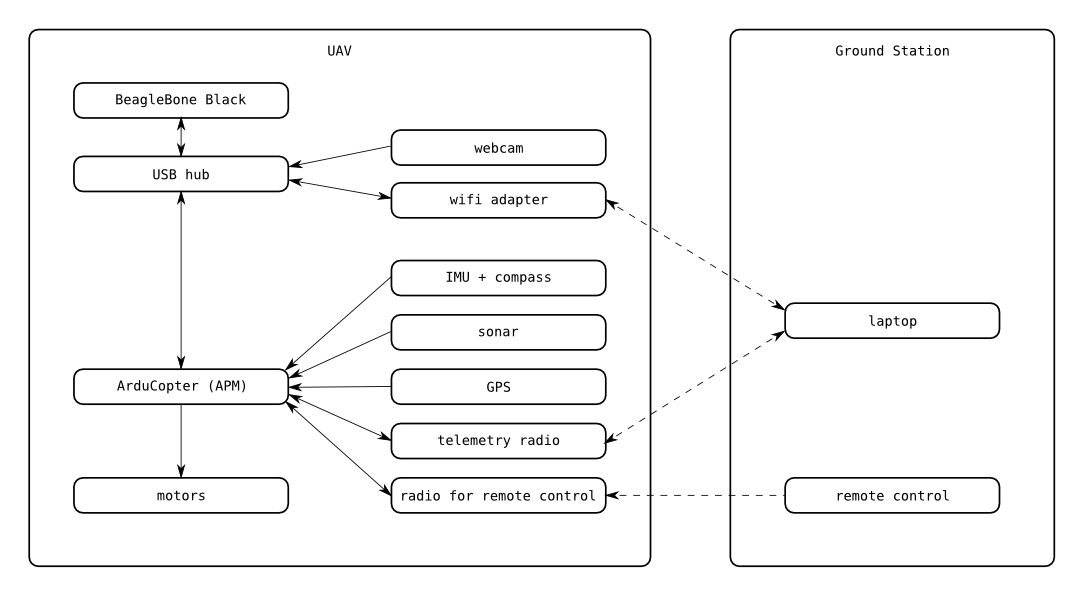
\includegraphics[width=\textwidth]{architecture.png}
    \caption{Proposed architecture of our automated landing system for UAVs}
    \label{fig:architecture}
\end{figure*}


%%%%%%%%%%%%%%%%%%%%%%%%%%%%%%%%%%%%%%%%%%%%%%%%%%%%%%%%%%%%%%%%%%%%%%%%%%%%%%
\section{Landing Accuracy with GPS Only}

Blarg.

%%%%%%%%%%%%%%%%%%%%%%%%%%%%%%%%%%%%%%%%%%%%%%%%%%%%%%%%%%%%%%%%%%%%%%%%%%%%%%
\section{Outline of Vision Approach}

After reading several papers on vision-based landing for UAVs, we decided to
emulate the approach by Sharp, Shakernia, and Sastry in their 2001 paper, ``A
Vision System for Landing an Unmanned Aerial Vehicle''. Our landing platform
will have an easy-to-detect geometric shape given by six red squares on a white
background. (We are building a cardboard prototype on Monday, November 18). Our
vision system will continuously try to estimate the camera's position w.r.t.
the landing platform. We will do this by first detecting the landing platform
in each frame (thresholding, segmentation, corner detection, and feature
labeling), and then estimating the pose of the camera (by solving a version of
the structure-from-motion problem in computer vision). Following Sastry et al,
we can use the onboard GPS + IMU to get an estimate of the quadcopter's pose,
and use this data to validate the vision-based pose estimate.

\end{document}
